\section{Hardware Design}

\subsection{Introduction}
This report presents a design for a standalone real-time stereo audio system that is capable of processing both speech and music. The selected components were chosen in order to provide high-quality audio while maintaining reasonable costs. Additional requirements include adequate debugging capabilities, and a memory to store the result of and accommodate a high-resolution FIR filtering process.\\


\subsection{Specifications}
The ADC and DAC resolution was chosen to be 16 bits as any higher resolution is considered imperceptible for a typical human ear \autocite{jackson2014}. This results in a SQNR of 96 dB - as per equation \ref{eq:sqnr}, which is more than the SNR of most CODECs. In order to maximize the available dynamic range, the minimal SNR of the CODEC was set to be at least 90dB.

\begin{equation}\label{eq:sqnr}
SQNR = 20\log_{10}(2^N)    
\end{equation}


A sampling frequency of 48 kHz is today’s industry standard for studio-quality music \autocite{AES48khz} and would also accommodate the Compact Disk standard of 16-bit Audio at a sampling frequency of 44.1 kHz. The minimal specifications for the DSP processor and the CODEC are summarized in tables \ref{tb:specsDSP} and \ref{tb:specsCodec} respectively.




\begin{table}[h]
	\centering
	\begin{tabular}{|l|l|}
		\hline
		\textbf{Sampling Frequency}            & 48kHz                            \\ \hline
		\textbf{Bitrate (per channel)}         & 16bit                            \\ \hline
		\textbf{Minimum number of filter taps} & 2048 (stereo)                    \\ \hline
		\textbf{Minimum number of MMACs}       & 200MMAC                          \\ \hline
		\textbf{Peripherals}                   & SPI, TWI, UART, PLL, GPIO, SPORT \\ \hline
	\end{tabular}
	\caption{DSP system minimal specifications requirements}
	\label{tb:specsDSP}
\end{table}

\begin{table}[h]
	\centering
	\begin{tabular}{|l|l|}
		\hline
		\textbf{Number of channels}            & 2 ADCs and 2 DACs (stereo)                           \\ \hline
		\textbf{Sampling Frequency}            & 48kHz                            \\ \hline
		\textbf{Bitrate (per channel)}         & 16bit                            \\ \hline
		\textbf{Minimum SNR} & 90dB (stereo)                    \\ \hline
		\textbf{Peripherals}                   & TWI, SPI or SPORT \\ \hline
	\end{tabular}
	\caption{CODEC minimal specifications requirements}
	\label{tb:specsCodec}
\end{table}

\subsection{DPS Processor}
For the signal processing, the DSP has to perform at least one full convolution per sample. At a sampling frequency of 48 kHz and a minimum number of 2048 taps per channel, this demands at least 200 MMACs. Thus the minimum specifications for the desired processor are listed in the Table \ref{tb:specsDSP}.\\

Based on these minimal requirements, the group has selected the Blackfin ADSP-BF592 DSP chip. At a price of only approximately £4, it features two 16-bit MACs operating at up to 400 MHz \autocite{blackfinDSP} . This would theoretically allow single channel, real-time filtering, using up to 8192 filter taps per sample. \\

Alternately, this surplus in computational power can be used for other processes. The chip possesses all necessary hardware communication peripherals in a DSP system. This includes the SPORT and TWI for sending and receiving data from the codec, SPI for stand-alone ROM booting, and UART and JTAG for communicating with the debugger. \\



\subsection{Codec}
The requirements for the codec is to provide ADC and DAC facilities at 16-bit resolution. However, a codec with a 24-bit resolution was found to be more economical. The main parameters considered were the dynamic range and the Signal-to-Noise ratio (SNR). Other feature requirements for the codec were a stereo-audio interface and SPI capabilities. \\

As a result, the ADAU1961 24-bit stereo audio codec with integrated PLL was chosen. At a price of £2.5 \autocite{digikeyCodec}, it has an SNR of 98 dB and communicates using both SPI and TWI \autocite{codec_datasheet}. These are essential for communicating with the flash ROM and receiving control signals from the DSP chip respectively.



\subsection{Memory}
The processor implements a modified Harvard architecture combined with a 2 level hierarchical memory structure \autocite{blackfinDSP}. This allows for high-speed processing of multiple datasets using pipelining. For the particular application of filtering, allowing the data and instructions to be accessed simultaneously.\\

The first memory level is implemented in a modified Harvard architecture. One region is allocated for instructions, and another 2 independent regions can be used to store vector data (such as real and imaginary vectors). The second level is intended to be a slower form of memory and thus is implemented in the Von Neumann architecture. This second level is intended to store data for non-speed-critical operations. Additional to the two levels, memory is to be reserved for the memory mapped control registers of peripherals. \\

Further to such a layered RAM structure, it is necessary for the Bootloader to be stored in non-volatile memory (flash ROM – via SPI Master). Doing so enables program instructions/firmware to be stored permanently within the system such that the device can operate as standalone from the point of power-on. Further to physically storing program instructions and firmware within the device, in order to accommodate rapid debugging, UART boot mode is to be supported.

\subsection{Interface with Codec}
Communication with the Codec is established through 2 peripherals: TWI and SPORT.\\ 

TWI is compatible with I2C, a standard protocol, and used for occasional control communications with Codec. TWI is bi-directional and runs at a lower frequency than the other peripheral connection: SPORT. 
A possible use-case for the TWI is the sharing of information regarding volume. The DSP System would query for volume levels by sending a protocoled message to the Codec, and the Codec would then reply with the volume data (contained in peripheral registers) after having received the information. \\

The SPORT implements the SPI framework for communication with the Codec. SPORT is used for passing digitized serial audio data that is going to be processed from the Codec into the DSP. After the DSP system has completed its processing of the audio signal, the resulting signal is fed back to the codec. 


\begin{figure}[h!]
	\centering
	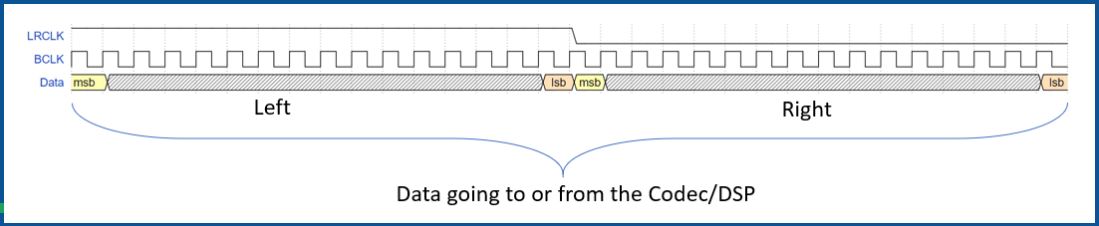
\includegraphics[width=\textwidth]{time.png}
	\caption{Timing diagram for Codec/DPS communication.}
	\label{fig:timing}
\end{figure}




\subsection{GPIO}
GPIO pins can be configured by the user at run-time through their respective control registers. The logic levels of the pins can be programmed to be edge-sensitive or level-sensitive. In some ways, the number of GPIO pins the system possesses reflects the flexibility of the system at hand. 


\begin{itemize}
	\setlength\itemsep{0.1em}
	\item Defining the I/O configuration of a given pin. 
	\item Managing control and status of a given signal/pin. 
	\item Configuring GPIO interrupts. 
\end{itemize}




\subsection{UART for interfacing with debugger}

The UART ports in the DSP system’s processor are used to interface the system with external hosts or interfaces for debugging, data transfer and communications. In addition to this, the UART can be used to boot-load the processor after launching or resetting it. This application, however, is dependent upon the boot mode pins’ configuration. 

\subsection{SPI and Flash memory}

The serial peripheral interface (SPI) provides the interface to the Flash memory for accessing the bootloader when operating in a standalone environment. SPI provides a mechanism to interface a high-speed system with external peripherals that run at lower clock speeds. Flash memory is non-volatile and electrically erasable. In the context of this DSP system, it would be used to store the operating system. Upon reset or system launch, the OS would then be read from the processor’s code memory before execution - making it standalone. 


\subsection{PLL}
Different parts of the DSP run at different clock rates. To deal with the difference in clock speeds in the system, a PLL can be used to localise the high-frequency operations of the processor. Different parts of the system inevitably run at a lower clock speed than the main processor. This is because if they would accommodate the clock speed of the main processor, resulting EM interference and noise would damage performance. Therefore, a PLL is required to maintain the clock speeds that minimise interference in the system’s different parts.\\  


The SPORT implementation can be described by the figure above. The transmission of the data and its synchronisation is driven by two clock signals: The Left-Right Clock (LRCLK) and the Bit Clock (BCLK). When the LRCLK transitions from logic 1 to logic 0 (or the opposite), a new stream of data from a channel is signalled to the DSP. The DSP will then read the data from the channels at a rate in-sync with the BCLK. In the system at hand, each channel is defined over 16 bits. The allocation of the SPORT follows Time Division Multiplexing as more than one channel is used in the system. 


\subsection{Real-Time DSP System}

\begin{figure}[h!]
	\centering
	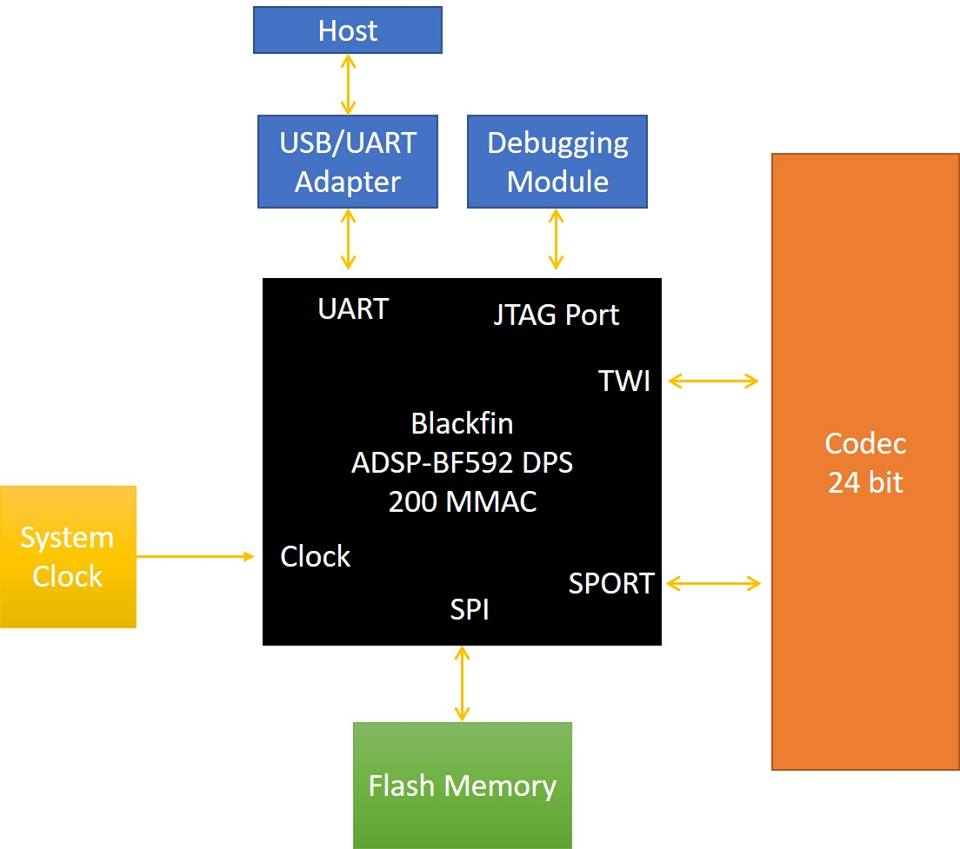
\includegraphics[width=0.5\textwidth]{diagram.jpg}
	\caption{Real-time DPS Design Block diagram.}
	\label{fig:block}
\end{figure}



\subsection{Conclusion}
This report examined the various design constraints and considerations involved when designing a Digital Signal Processing system. The report first began with an outline of the main requirements a DSP system needs to meet to match industry standards. Based on these definitions, a processor model was proposed and its main characteristics were described. The following is a summary of the chosen parameters for the proposed system. 


\begin{itemize}
	\setlength\itemsep{0.1em}
	\item ADSP-BF592 DSP device, operating at 200MMAC (16 bit)
	\item External clocking system 
	\item UART interface for boot mode and serial connection to computer 
	\item Serial flash memory to hold the operating system, connected to the SPI 
	\item ADAU1961 24-bit stereo codec, connected to TWI (control) and SPORT (audio data)
	\item JTAG debugging interface
\end{itemize}
